\section{Kolväten}
Kolväten är organiska ämnen som är föreningar av enbart kol och väte. Det finns dock många ämnen som innehåller några enstaka extra ämnen som fortfarande räknas som kolväten, exempelvis alkoholer med en OH-grupp. Kolvätens struktur betecknas på två olika sätt. Antingen med traditionella strukturformler eller s.k. streckformler. En streckformel är till för att spara plats på papperet. Kolväten ritas upp i ett sick-sack-streck där varje hörn är en kolatom. Om det finns förgreningar eller andra avvikelser från den mest grundläggande formen av kolväten kommer det att ritas in. Här följer några exempel:
\begin{center}
    \begin{tabular}{c >{\hspace{20pt}}c >{\hspace{20pt}}c}
        \chemfig{H-C([2]-H)([-2]-H)-C([2]-H)([-2]-H)-H} & \chemfig[angle increment=30]{-[1]-[-1]-[1]} & \chemfig[angle increment=30]{-[1]=[-1]([:-90]-OH)-[1]} \\ \vspace{5pt} \\
        Strukturformel & Streckformel & Streckformel med avvikelser
    \end{tabular}
\end{center} 
Dessa är dock alla tvådimensionella diagram och molekylernas strukctur är faktiskt tredimensionell. Detta är ett exempel på den tredimensionella strukturen på $\ce{CH4}$ (metan):
\begin{center}
    \chemfig{H-[:30]C([:-50]<H)([:-20]<:H)-[:90]H}
\end{center}
På denna bild innebär \raisebox{3pt}{\chemfig{<[,0.5]}} att en atom ligger ''framför'' dess bundna partner medan \raisebox{3pt}{\chemfig{<:[,0.5]}} innebär att den är ''bakom''. Detta bildar då en tetraeeder i 3D och varje bindning har en vinkel av $109.47^\circ$ mellan varandra. Denna tetraederformation är standard för kolatomer och alla köfreningar försöker att upprätthålla kolets bindningsmönster. Detta leder til de sick-sackiga bindinigsmönstren som vi ser i kolväten och andra kolföreningar.
\subsection{Alkaner}
Alkaner är konväten som innehåller enbart enkla kovalenta bindningar mellan atomerna. De första 10 heter och ser ut som följande:
\begin{center}
    \tcbox[title={De 10 första - namn}]{\begin{tabular}{r c l}
            1. & Metan & \ce{CH4} \\
            2. & Etan & \ce{C2H6} \\
            3. & Propan & \ce{C3H8} \\
            4. & Butan & \ce{C4H10} \\
            5. & Pentan & \ce{C5H12} \\
            6. & Hexan & \ce{C6H14} \\
            7. & Heptan & \ce{C7H16} \\
            8. & Oktan & \ce{C8H18} \\
            9. & Nonan & \ce{C9H20} \\
            10. & Dekan & \ce{C10H22}
    \end{tabular}}
    \tcbox[title={De 10 första - struktur}]{\begin{tabular}{c >{\hspace{20pt}}c >{\hspace{20pt}}c}
        \chemfig{H-C([-2]-H)([2]-H)-H} & \chemfig{H-C([-2]-H)([2]-H)-C([-2]-H)([2]-H)-H} & \chemfig{H-C([-2]-H)([2]-H)-C([-2]-H)([2]-H)-C([-2]-H)([2]-H)-H} \\ \vspace{5pt} \\
        Metan & Etan & Propan
    \end{tabular}}
\end{center}
Dessa är mycket bra att komma ihåg. De första fyra är gaser vid rumstemperatur medan de andra är vätskor. Utöver detta finns inget särskilt med dem i denna kurs.

\subsection{Alkener}
Samma sak som alkaner fast med minst en dubble kovalent bindning. Namnen är samma som alkaner fast en suffix -en läggs till, alltså met\underline{en}, et\underline{en} osv.

\subsection{Alkyner}
Återigen samma som alkaner fast med minst en trippel kovalent bindning. Namnen är samma fast med suffixen -yn, alltså met\underline{yn}, et\underline{yn} osv.

\subsection{Förgreningar}
\label{sec:grenar}
Ett kolväte kan förgrena sig och få avvikelse från dess mest grundläggande form. Detta kan vara i form av flera kolatomer, en OH-grupp eller något av de många andra möjlighetererna. En förgrening ritas precis som vanligt på streckformeln. Här följer några exempel:

\subsubsection*{Kolkedjor}
När ett kolväte förgrenar sig med andra kolväten ritas bara vanliga streck. Exempelvis:
\begin{center}
    \chemfig{-[1]-[-1]-[1](-[2]-[1])-[-1]-[1]-[-1]}
\end{center}
Föregrening har ett namn, i exemplet ovan är det en etylgrupp. Namnen är samma som motsvarande alkan fast med en -yl ändelse så met\underline{yl}grupp för en avgrenad kol, prop\underline{yl}grupp för tre stycken osv. Dubbel- och trippelbundna kolvätegrenar finns, men de kommer vi inte riktigt behöva arbeta med.

\subsubsection*{OH-grupper}
En gren kan också vara en \emph{hydroxidgrupp} (OH-grupp). Dessa ritas ut med atomerna insatta (se nedan). När en OH-grupp finns bildas en alkohol.
\begin{center}
    \chemfig{-[1]-[-1](-[-2]OH)-[1]}
\end{center}

\subsubsection*{Andra ämnen}
Alla andra icke-kol ämnen ritas precis som en OH-grupp och är inte en del av kursen för tillfället.

% TODO: add section about naming hydrocarbons

\subsection{Isomerer}
En \emph{isomer} är en kolförening som har samma summaformel som en annan men har en anna struktur rent fysiskt. Isomerer kan bildas på många olika sätt men de främsta vi ska titta på är förgreningar, cis- och transisomerer, multipelbindningar och cykliska kolväten. Viktigast att komma ihåg är nog att spegelbilder av en specifik kolkedja inte är en isomer, det är en ''pannkaka'' som Tor brukar säga.

\subsubsection{Förgreningar}
Först av allt, läs \cref{sec:grenar}. Förgrenade kolföreningar (kolväten i denna kurs) kan enbart vara isomerer av sig själva om deras summaformel är samma, dvs. att totalt antal väte- och kolatomer är konstant. So exempelvis butan är en isomer till 2-metylpropan:
\begin{center}
    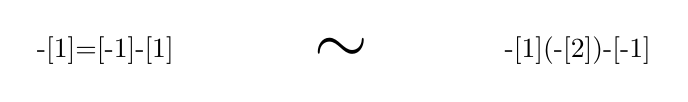
\begin{tikzpicture}
        \node at (0,0) {\Huge{$\sim$}};
        \node at (-3,0) {\chemfig{-[1]=[-1]-[1]}};
        \node at (3,0) {\chemfig{-[1](-[2])-[-1]}};
    \end{tikzpicture}
\end{center}
Detta kan vi se för att båda ha summaformeln \ce{C4H10}. Man räknar helt enkelt den totala antalet av varje atom (även de som inte är C/H) för att avgöra om grenade kolföreningar är isomerer.

\subsubsection{Cis- och transisomerer}
En kolatom som är bundet enkelt till en annan kolatom har förmågan att snurra sin bindning. Detta innebär att den 3-dimensionella strukture kan i verkligheten vara lite vad som helst:
\begin{center}
    \begin{tabular}{>{\centering\arraybackslash}m{0.2\textwidth} >{\centering\arraybackslash}m{0.1\textwidth} >{\centering\arraybackslash}m{0.2\textwidth} >{\centering\arraybackslash}m{0.1\textwidth} >{\centering\arraybackslash}m{0.2\textwidth}}
        \chemfig{-[1]-[-1]-[1]} & \Huge{$\sim$} & \chemfig{-[1]-[3]-[5]} & \Huge{$\sim$} & \chemfig{--[-1]-[1]}
    \end{tabular}
\end{center}

\subsection{Arener}
En aren, alternativt ett aromatisk ämne, är ett cykliskt kolväte som binder med varannan binding dubbel. I mitten av denna ring kommer då elektronerna alltid att enbart kunna anta två olika konfigurationer. Detta leder till att de \emph{delokaliseras} och bildar ett ''medelvärde'' av deras positioner sen innan. De kommer alltså att finnas typ som ett samlat moln för alla kolatomer, likt en metallbindning. Det ser ut som följande för en hexanbas:
\begin{center}
    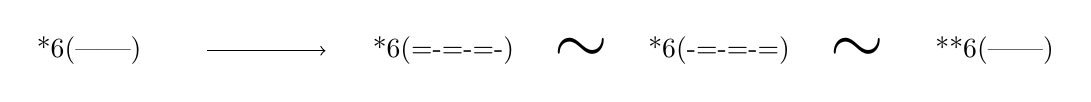
\begin{tikzpicture}
        \node at (-2.25,0) {\chemfig{*6(------)}};
        \draw[->] (0,00) ++(-1.5/2,0) -- ++(1.5,0);
        \draw (2.25,0) node {\chemfig{*6(=-=-=-)}} ++(2-0.25,0) node {\Huge{$\sim$}} ++(2-0.25,0) node {\chemfig{*6(-=-=-=)}} ++(2-0.25,0) node {\Huge{$\sim$}} ++(2-0.25,0) node {\chemfig{**6(------)}};
    \end{tikzpicture}
\end{center}

I detta fall innebär $\sim$ att något är samma molekyl som något annat. Denna aren för hexan kallas \emph{bensen}. Ringen i mitten ska illustrera detta medelvärde av elektroner och visar helt enkelt att det är ett aromatiskt ämne. Ett annat intressant aromatiskt ämne är \emph{grafen} vilket är en stor platta av sammanvävna kol-hexagoner med aromatiska bindningar som sedan har en kant av väte. Detta ser ut såhär:
\begin{center}
    \scalebox{0.8}{\chemfig[angle increment=30]{**6(([-3]**6(--([-5,0.5]-H)-([-3,0.5]-H)---))-(**6(--([-3,0.5]-H)-([-1,0.5]-H)---))-(**6(--([-1,0.5]-H)-([1,0.5]-H)---))-(**6(--([1,0.5]-H)-([3,0.5]-H)---))-(**6(--([3,0.5]-H)-([5,0.5]-H)---))-(**6(--([5,0.5]-H)-([7,0.5]-H)---))-)}}
\end{center}
I verkligheten expanderar detta mycket större, men i brist på plats är detta en lite del av en hypotetisk grafenskiva. Väte kommer enbart uppstå längs med kanterna på skivan.